\documentclass[11pt,a4paper]{article}

\usepackage[T1]{fontenc}
\usepackage[utf8]{inputenc}
\usepackage[english]{babel}
\usepackage[a4paper,margin=2.4cm]{geometry}
\usepackage{booktabs}
\usepackage{enumitem}
\usepackage{parskip}
\usepackage{csquotes}
\usepackage{graphicx}
\usepackage[hidelinks]{hyperref}

\hypersetup{colorlinks=false,
  pdftitle={DiLab Foresight Sprint 5 Documentation},
  pdfauthor={Paul Keck}}

% ---- notes (plain run-in, no colour) -------------------------------------
\newcommand{\note}[2]{\par\smallskip\noindent\textbf{#1.}\enspace #2\par\smallskip}
\newcommand{\key}[2]{\note{#1}{#2}}
\newcommand{\warnb}[2]{\note{#1}{#2}}
\newcommand{\tipb}[2]{\note{#1}{#2}}
\newcommand{\code}[1]{\texttt{\small #1}}
\newcommand{\refitem}[1]{\par\noindent\hangindent=1.5em\hangafter=1 #1\par\smallskip}

\pagestyle{plain}

\setlist[itemize]{leftmargin=1.4em, itemsep=2pt, topsep=3pt}
\setlist[enumerate]{leftmargin=1.6em, itemsep=2pt, topsep=3pt}

\title{\vspace{-1.2cm}\textbf{Sprint 5 Documentation: \enquote{Final Polish}}\\[4pt]
  \large AI-Driven Scaling of Strategic Technology Foresight}
\author{Paul Keck \quad\textit{(Scrum Master, Sprint 5)}}
\date{Sprint 5: 22 June to 6 July 2026}

\begin{document}
\maketitle
\thispagestyle{plain}

\vspace{-4mm}
\begin{center}\small
\textbf{Course:} Digital Innovation Lab / Management \& Digital Technologies II (LMU) \quad\textbar\quad
\textbf{Partner:} Rohde \& Schwarz (PO: Dr.\ Andrew Schaefer)\\
\textbf{Team 2:} Christian Diogo Götsch, Paul Keck, Aditya Purwar, Lovepreet Singh, Adam Foster-Baird
\end{center}

\begin{abstract}
\noindent Sprint~5 was the last content sprint before the closing presentations, and the aim was to take a
working research prototype to a finished state. The team committed 55 story points across nine stories and
completed 52; one story, the R\&S local-inference integration, was blocked outside the team and carried
over. The sprint also produced work that was never on the committed backlog, mainly the archetype and
hybrid-structure analysis and the code that generates it, and that turned out to be the sprint's main
technical result. This document covers the product and sprint backlogs, the burndown, the sprint review, the
story-point estimate against the outcome, the Scrum process and retrospective, the theoretical background,
the results and their interpretation, the limitations and outlook, and the source code.
\end{abstract}

\tableofcontents
\vspace{3mm}

% =========================================================================
\section{Product Backlog}
The product is a domain-agnostic foresight engine: it ingests a knowledge base and derives a map of
plausible futures for whatever domain that base describes. Regulatory spectrum monitoring, the
Rohde~\&~Schwarz field, is the running test case; the reusable engine itself is the deliverable. The backlog
below is organised as nine epics along the pipeline, followed by a forward-looking backlog. Titles are
reconstructed from the Jira project (\code{DFF}, board~34) and the codebase, so the exact wording may differ
from the board.

\begin{center}\small
\begin{tabular}{@{}lll@{}}
\toprule
\textbf{Epic} & \textbf{Title} & \textbf{Status} \\
\midrule
DFF-2 & Knowledge base \& RAG ingestion (Chroma vector DB) & ongoing \\
DFF-3 & BOM product decomposition (response drivers) & done \\
DFF-4 & Trend scanning \& driving-driver extraction (4 dimensions) & done \\
DFF-5 & Driver merge \& morphological (Zwicky) box & done \\
DFF-6 & CIB cross-impact elicitation (persona panel + Delphi) & done \\
DFF-7 & Scenario generation (fixed-point + combinatorial) & done \\
DFF-8 & Structure \& archetype analysis & done (this sprint) \\
DFF-9 & Evaluation: MCDA (AHP/TOPSIS), temporal, strategic framing & done \\
DFF-10 & Dashboard, UI \& delivery & done (this sprint) \\
\midrule
\multicolumn{3}{@{}l}{\textit{Future backlog}}\\
DFF-23 & Enrich the (thin) geopolitical corpus dimension & to do \\
DFF-24 & MCDA score anchoring / de-compress evaluation scores & to do \\
DFF-25 & Complete R\&S local-inference endpoint integration (continues S7) & to do \\
DFF-26 & Human-in-the-loop / stronger-model CIB validation & to do \\
\bottomrule
\end{tabular}
\end{center}

% =========================================================================
\section{Sprint Backlog}
These are the nine stories committed for Sprint~5 (sprint board \code{DFF}, sprint id~69). The
\enquote{Status @ 28 Jun} column is the mid-sprint checkpoint that anchors the burndown.

\begin{center}\small
\begin{tabular}{@{}lllcl@{}}
\toprule
\textbf{Key} & \textbf{Story} & \textbf{Assignee} & \textbf{SP} & \textbf{Status @ 28 Jun} \\
\midrule
DFF-11 & S1 · Make pipeline domain-agnostic        & Paul      & 8 & Done \\
DFF-12 & S2 · Fix positivity bias (split-scoring)  & Christian & 8 & Done \\
DFF-13 & S3 · Null-model significance test         & Aditya    & 5 & Done \\
DFF-17 & S7 · Connect R\&S local inference endpoints & Paul    & 3 & To Do \\
DFF-18 & S8 · ML technology-driver extraction      & Aditya    & 8 & In Progress \\
DFF-19 & S9 · Polish UI                            & Adam      & 5 & In Progress \\
DFF-20 & S10 · LLM-as-a-Judge evaluation layer     & Lovepreet & 8 & In Progress \\
DFF-21 & S11 · Domain-agnostic on agriculture corpus & Christian & 5 & In Progress \\
DFF-22 & S12 · Refine contrastive CCA              & Paul      & 5 & In Progress \\
\midrule
\multicolumn{3}{@{}l}{\textbf{Committed}} & \textbf{55} & \\
\multicolumn{3}{@{}l}{Done by 28 Jun} & 21 & \\
\bottomrule
\end{tabular}
\end{center}

% =========================================================================
\section{Burn-down Chart}
\begin{figure}[h]
\centering
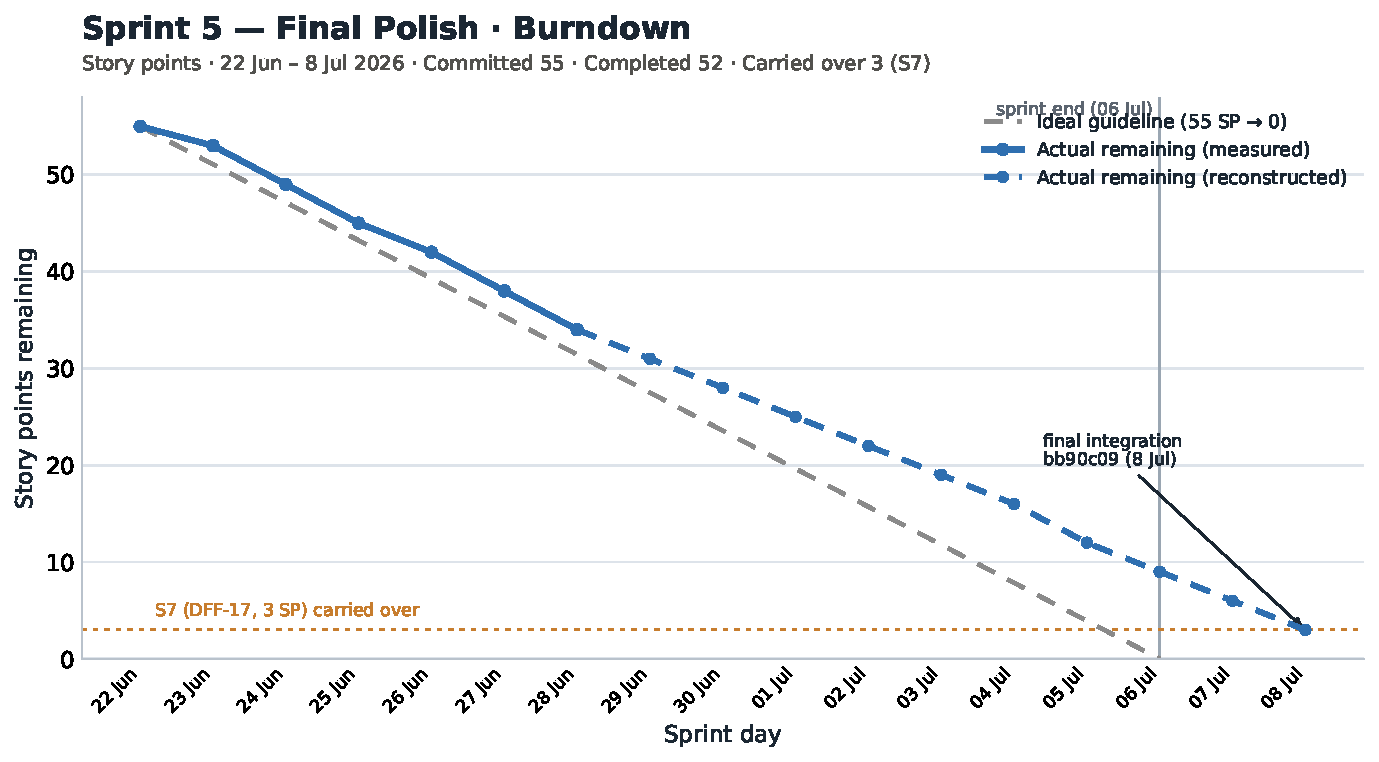
\includegraphics[width=0.95\linewidth]{sprint5_burndown.pdf}
\caption{Sprint~5 burndown (story points). The actual line is measured for 22--28 June
(Sprint5\_Burndown.xlsx) and reconstructed from commit landing dates afterwards. It stays close to the ideal
guideline and clears on 8 July with the finalisation commit \code{bb90c09}, two days after the official
sprint end (6 July). It stops at 3~SP because story~S7 (DFF-17) carried over. Of the 55 committed points, 52
were completed.}
\end{figure}

The actual line stays close to the ideal guideline through the sprint. Its last points are reconstructed
from commit landing dates: the remaining stories were merged in the finalisation commit \code{bb90c09} on
8 July, two days past the official sprint end, which the retrospective (Section~\ref{sec:process}) picks up
as a late integration. The team completed 52 of the 55 committed points; S7 (DFF-17, the R\&S local-inference
endpoints) was blocked externally and carried over.

% =========================================================================
\section{Sprint Review}
\subsection*{Sprint goal}
The goal was to bring the prototype to a finished product: repair the remaining quality problem in the
cross-impact step, make the engine reusable across domains, and get the analysis behind a dashboard in time
for the final presentations. The items below explain the reasoning behind each piece of work as well as what
it does.

\subsection*{What was delivered}
Ownership is noted per item; the committed backlog was spread across the whole team.
\begin{itemize}
  \item \textbf{ML technology-driver extraction (S8, Aditya Purwar).} Aditya built an arXiv ingestion
  pipeline that pulls candidate technology drivers straight from the research literature with an ML/NLP
  stage. It complements the manual bottom-up BOM decomposition and grows the driver base on its own, so the
  driver set scales with the corpus instead of with analyst time. That is what the domain-agnostic goal
  needs: a new field should not require a fresh round of manual driver-hunting.
  \item \textbf{LLM-as-a-Judge evaluation layer (S10, Lovepreet Singh).} Lovepreet added an evidence-grounded
  auditor that scores each scenario and cites the source passages behind every score, then feeds those
  scores into the multi-criteria ranking (AHP weights, TOPSIS). R\&S treats traceability
  (\enquote{Nachvollziehbarkeit}) as a hard requirement, so a score the model simply asserts is not enough;
  it has to point back to the corpus.
  \item \textbf{Cross-impact quality fix (S2, Christian Götsch).} Language models lean positive. Asked
  whether two technologies can coexist, they almost always say yes, so the earlier cross-impact matrix
  carried hardly any trade-offs and the scenario space collapsed onto a single consensus future. Hand-tuning
  the prompt is brittle and tends to overshoot into fake pessimism, so Christian changed the aggregation
  instead: a strong minority trade-off is now kept in the panel result rather than smoothed out by the
  median. The share of negative couplings rose from 2\% to 29\%, inside the 20--30\% band reported for real
  CIB matrices (Weimer-Jehle 2006).
  \item \textbf{Domain-agnostic engine (S1, S11; Paul Keck and Christian Götsch).} The demo topic was
  hard-coded in about fifteen places, so any other corpus produced nonsense. The Product Owner had made
  clear that the deliverable is a reusable framework, so the flow was turned around: the engine reads the
  corpus first, works out the domain profile itself, and passes that to every later step. A guard test fails
  the build if a domain term creeps back into the code. Docking an unrelated corpus on agriculture and field
  robotics produced a coherent analysis with no code changes.
  \item \textbf{Null-model significance test (S3, Aditya Purwar).} A scenario study only carries weight if
  the question \enquote{are there distinct scenario families?} gets an evidence-based answer. Aditya's test
  compares the real field against a uniform-random field of the same shape and returns a significance ($z$)
  score, so the claim rests on a number instead of a hunch.
  \item \textbf{Dashboard and UI (S9, Adam Foster-Baird).} Adam's React/FastAPI dashboard shows the
  landscape, the named archetypes, and the multi-method structure comparison next to each other, so a
  non-technical stakeholder can work through the result without opening a JSON file.
\end{itemize}

\subsection*{Main result}
The main finding (Section~\ref{sec:results}) is that the scenario field is a hybrid. A dense core of a few
well-separated scenario families sits inside a continuum, where the rest of the field shades gradually from
one case to the next. Standard clustering misses the core; a density method on an ordinal encoding brings it
out. Running the same method on a synthetic field that does contain real structure recovers clean clusters,
which is why the \enquote{mostly-continuum} verdict on the real field reads as a feature of the domain: the
tool finds structure when structure is there.

\subsection*{Review meeting with the Product Owner}
The increments were shown to the Product Owner, Dr.\ Andrew Schaefer (R\&S), at the sprint review. He
accepted the domain-agnostic engine and the cross-domain demonstration on the agriculture corpus as the main
increment of the sprint, and repeated his earlier steer: the reusable framework is what matters to him, and
the spectrum results stay a test case. He again put weight on traceability, that every driver and scenario
has to point back to a source. Two things followed for the backlog. First, keep hardening the framework's
generality and its evidence trail. Second, treat spectrum-specific polish as lower priority. The open R\&S
local-inference integration (S7) was noted as blocked on his side and moved to the next sprint.

% =========================================================================
\section{Story-Point Estimation vs.\ Reality}
Eight of the nine committed stories were finished. Only S7 carried over, blocked on an external R\&S
endpoint, and it has no commit because the dependency never arrived.

\begin{center}\small
\begin{tabular}{@{}llccl@{}}
\toprule
\textbf{Key} & \textbf{Story} & \textbf{Committed} & \textbf{Completed} & \textbf{End status} \\
\midrule
DFF-11 & S1 · Domain-agnostic pipeline      & 8 & 8 & Done \\
DFF-12 & S2 · Positivity-bias fix           & 8 & 8 & Done \\
DFF-13 & S3 · Null-model test               & 5 & 5 & Done \\
DFF-17 & S7 · R\&S local inference endpoints & 3 & 0 & \textbf{Carried over} \\
DFF-18 & S8 · ML technology-driver extraction & 8 & 8 & Done \\
DFF-19 & S9 · UI polish                     & 5 & 5 & Done \\
DFF-20 & S10 · LLM-as-a-Judge layer         & 8 & 8 & Done \\
DFF-21 & S11 · Agriculture-corpus proof     & 5 & 5 & Done \\
DFF-22 & S12 · Contrastive CCA refinement   & 5 & 5 & Done \\
\midrule
& \textbf{Total} & \textbf{55} & \textbf{52} & 3 carried over \\
\bottomrule
\end{tabular}
\end{center}

\subsection*{Scope delivered beyond the commitment}
The sprint also took on work that was never on the committed backlog, mostly the archetype and continuum
analysis and the code needed to establish it. None of it was estimated in advance. A rough sizing after the
fact comes to about \textbf{39~SP}:

\begin{center}\small
\begin{tabular}{@{}lc l@{}}
\toprule
\textbf{Unplanned work delivered} & \textbf{$\approx$SP} & \textbf{Landed in} \\
\midrule
Archetype module (HDBSCAN+ordinal, LLM-named clusters, continuum halo) & 13 & \code{bb90c09} \\
Multi-method structure comparison + structure referees & 8 & \code{2d1583b} \\
Temporal / DVI signal-maturity module & 5 & \code{34e08ba} \\
\code{run\_full.py} one-command orchestrator & 5 & \code{bb90c09} \\
Corpus enrichment (arXiv + report PDFs) + engine-soundness validation & 5 & \code{43969d2} \\
LLM infra hardening (pooled model, timeouts, retry) & 3 & \code{bb90c09} \\
\midrule
\textbf{Total unplanned} & \textbf{$\approx$39} & \\
\bottomrule
\end{tabular}
\end{center}

\key{Estimation reflection}{The committed 55~SP were mostly met, with 52 completed, but a similar amount of
unplanned work was absorbed without ever being planned. That points to a planning miss: exploratory scope
was under-counted and should have gone onto the board as estimated stories while it was happening. The
retrospective (Section~\ref{sec:process}) lists the corrective actions.}

% =========================================================================
\section{Scrum Process \& Retrospective}\label{sec:process}
\subsection*{Roles}
Following the course model, the team rotates the Scrum Master role each sprint. Paul Keck held it for
Sprint~5 and owns this documentation. The Product Owner is external (Dr.\ Andrew Schaefer, R\&S), and the
other members work as a self-organising development team.

\subsection*{Release strategy}
Work is integrated on the \code{feature/combinatorial-landscape} branch and checked by a
continuous-integration workflow that runs \code{pytest} on every push. The definition of done for the
sprint increment is a runnable pipeline plus dashboard: the whole analysis reproduces from one command
(\code{run\_full.py}), and the React front-end builds against the FastAPI back-end. Story points count as
burned only once a story's code has landed and its tests pass. Results are seeded so runs reproduce, and
every claim traces back to source passages through propagated \code{source\_chunk\_ids}.

\subsection*{Cadence \& attendance}
Sprint~5 ran on two whole-team meetings, one for planning at the start and one for the review and
retrospective at the end, plus a bi-daily stand-up every second day. Attendance at the stand-ups was uneven:
three or fewer of the five members usually joined, and on two of them only the Scrum Master showed up. The
Jira board (\code{DFF}) acted as the asynchronous record so absent members could pick up status without a
live meeting.

\subsection*{Work distribution}
The committed backlog was owned across the team: Aditya Purwar (ML technology-driver extraction, null-model
test), Lovepreet Singh (LLM-as-a-Judge evaluation layer), Christian Götsch (cross-impact de-biasing,
agriculture-corpus proof), Adam Foster-Baird (dashboard and UI), and Paul Keck (domain-agnostic core,
contrastive CCA). The extra, unplanned work of about 39~SP was carried mostly by the Scrum Master with AI
assistance. Concentrating it on one person is a bus-factor risk, which the retrospective picks up below.

\subsection*{Retrospective}
\begin{itemize}
  \item \textbf{What went well.} The mid-sprint scope clarification with the PO saved weeks of effort on the
  wrong deliverable. The dissent-preserving CIB fix and the engine-soundness check settled two open worries
  with measured numbers. The one-command orchestrator made the pipeline easy to demonstrate end to end.
  \item \textbf{What to improve.} Stand-up attendance was thin, twice down to the Scrum Master alone, and
  coordination suffered for it. Too much of the unplanned scope landed on one person, which is a bus-factor
  risk for a team deliverable. Estimation under-counted the exploratory work, which produced a large overrun
  and a late integration crunch. And one committed story (S7) hung on an external party, so it should have
  been marked blocked at planning rather than committed.
  \item \textbf{Actions for the next sprint.} Protect a fixed stand-up slot and ask for a written async
  update from anyone who cannot attend. Pair on the analysis modules so knowledge is not siloed. Set aside
  explicit capacity for discovery and open stories for it as it appears. Keep externally blocked items off
  the commitment until the dependency is available.
\end{itemize}

% =========================================================================
\section{Theoretical Foundation}\label{sec:theory}
The pipeline puts together established foresight and decision methods with current NLP, and each step rests
on a method with a track record.

\textbf{Scenario planning and foresight.} The work sits in the tradition of exploratory scenario planning
(Schwartz 1991; Kosow \& Gaßner 2008; Amer et al.\ 2013), which lays out several internally consistent,
plausible futures to support decisions under deep uncertainty.

\textbf{Morphological analysis.} The space of futures comes from a morphological box (the \enquote{Zwicky
box}): a small set of drivers, each with a few ordered states, whose combinations define scenarios (Zwicky
1969; Ritchey 2011). The states are kept ordinal (optimistic~$\to$~pessimistic) so that later analysis can
use their order.

\textbf{Cross-Impact Balance (CIB).} Not every combination is coherent. Following Weimer-Jehle (2006), a CIB
matrix records for each pair of driver states whether one promotes or inhibits the other, and consistent
scenarios are the ones with low internal tension. We elicit the matrix from a panel of LLM personas over two
Delphi-style rounds and keep dissent in the aggregation, since LLMs carry a documented positivity and
sycophancy bias (Sharma et al.\ 2023) that would otherwise erase the trade-offs.

\textbf{Retrieval-augmented generation.} Every generative step draws on retrieved source passages (Lewis et
al.\ 2020), which keeps the narratives tied to the corpus and makes them traceable.

\textbf{Structure analysis.} To judge whether distinct scenario families exist, we use the silhouette
coefficient (Rousseeuw 1987) against a uniform-random null model, and we set a partitioning method (KMeans)
beside a density method that can leave points unassigned (HDBSCAN; Campello et al.\ 2013). Layouts are drawn
with UMAP (McInnes et al.\ 2018).

\textbf{Multi-criteria evaluation.} Scenarios are scored on several criteria and ranked with the Analytic
Hierarchy Process for the criterion weights (Saaty 1980) and TOPSIS for the ranking (Hwang \& Yoon 1981).

% =========================================================================
\section{Results}\label{sec:results}
\subsection{Scenario structure: before and after}
The main deliverable is a map of the scenario space together with an assessment of how much structure it
actually has. Under the standard lens, one-hot encoding with KMeans, every point is forced into some cluster
and the 120 combinatorial scenarios come out as a single cloud (silhouette about 0.07, which is the
random-null floor). Switching to a density method on an ordinal encoding (HDBSCAN, which is allowed to leave
points unassigned) pulls out a dense core of five named archetypes at a core silhouette of about 0.38, with
roughly a third of the field left as a continuum halo.

\warnb{Read the two silhouettes correctly}{The 0.07 (KMeans over all points) and the 0.38 (HDBSCAN over the
dense core only) are not the same measurement, so they should not be sold as a \enquote{0.07 to 0.38
improvement}. Put plainly: the standard lens hides a core that the right lens brings out, and about a third
of the field really is a continuum.}

\begin{figure}[ht]
\centering
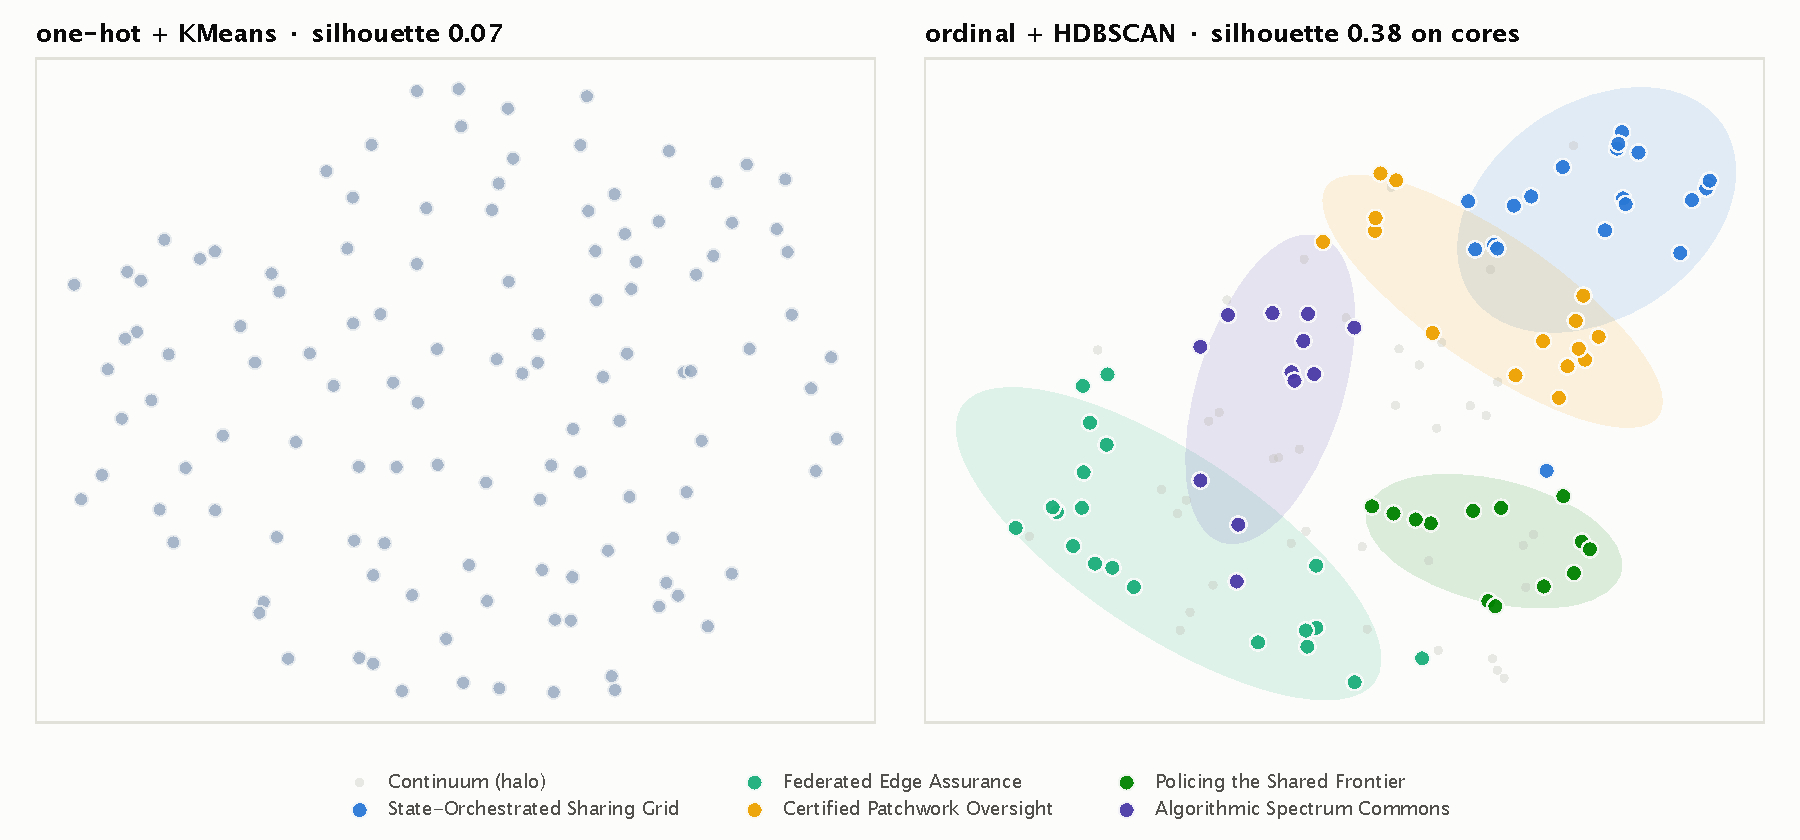
\includegraphics[width=\linewidth]{report_figures/space_two_lenses.pdf}
\caption{The scenario space under two lenses (the same 120 scenarios). Left: the standard view (one-hot with
KMeans) forces every point into a cluster, so the field reads as a single cloud (silhouette 0.07). Right: a
density method on the ordinal encoding (HDBSCAN) isolates five dense archetypes (core silhouette 0.38) and
leaves about a third of the field as a grey continuum halo.}
\end{figure}

The five archetypes on the spectrum test case are \textbf{State-Orchestrated Sharing Grid} (20 scenarios),
\textbf{Federated Edge Assurance} (20), \textbf{Certified Patchwork Oversight} (15), \textbf{Policing the
Shared Frontier} (13), and \textbf{Algorithmic Spectrum Commons} (12); the remaining 40 make up the
continuum.

\subsection{Engine validation: the standard-matrix control}
To check whether the \enquote{mostly-continuum} verdict says something about the domain or points to a
limitation of the tool, the same clustering engine was run on a standard, ground-truth CIB matrix. This is a
synthetic 8-driver matrix with two deliberately antagonistic blocks, where couplings promote within a block
and inhibit across blocks. It stands in for the textbook gold-standard check in a form that is offline and
deterministic. An uncoupled random matrix and the real spectrum field were run beside it:

\begin{center}\small
\begin{tabular}{@{}lcccl@{}}
\toprule
\textbf{Field} & \textbf{Silhouette} & \textbf{$z$-score} & \textbf{Eff.\ dim} & \textbf{Verdict} \\
\midrule
Standard matrix, coupled (positive control)   & \textbf{0.72} & 8.6  & 2.5  & usable structure \\
Standard matrix, uncoupled (negative control) & 0.22 & $-0.7$ & 7.8  & $\approx$ uniform random \\
Real spectrum field (14 drivers, 120 scenarios)  & 0.07 & 1.4  & 30.0 & $\approx$ uniform random \\
\bottomrule
\end{tabular}
\end{center}

\key{What the control shows}{On a matrix that really does contain structure the engine returns a clean
silhouette of 0.72 ($z=8.6$); on a random matrix it returns no usable structure ($z=-0.7$). The engine reads
the input for what it is, so the low separability of the real field reads most naturally as a feature of the
spectrum domain itself.}

\begin{figure}[ht]
\centering
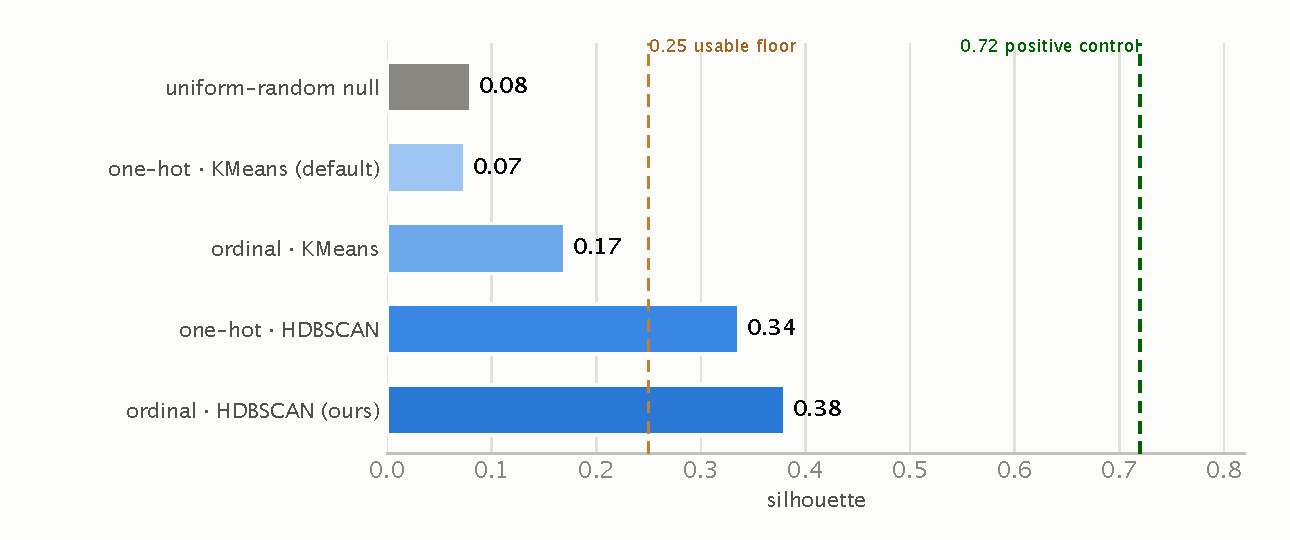
\includegraphics[width=0.9\linewidth]{report_figures/silhouette_by_lens.pdf}
\caption{Silhouette of the same field under five lenses, with the 0.25 usable-cluster floor and the 0.72
synthetic positive control marked. The default lens (one-hot with KMeans) sits at the random-null floor;
only the density method on the ordinal encoding clears the usable bar, and it is the same engine that
reaches 0.72 on a field with real structure.}
\end{figure}

Two further measurements point the same way. A null-model test on the real combinatorial field gives
$z=2.62$ for the silhouette, which is above random noise but still below the 0.25 usable-cluster floor,
exactly the hybrid picture. The CIB de-biasing moved the negative-coupling share from 2\% under the
positivity-biased setup to 29\% under dissent-preserving aggregation, inside the literature's 20--30\% band.
A contrastive elicitation prompt was also tried; it did not reliably raise the negative share, because the
current drivers are largely complementary, and that negative result is reported here as well.

\subsection{Interpretation \& discussion: what it means for R\&S}
Each archetype describes a different world, and taken together they point to a few concrete implications:
\begin{itemize}
  \item \textbf{State-Orchestrated Sharing Grid:} regulators run dynamic spectrum sharing from the centre.
  That plays to regulator-grade monitoring and enforcement, an R\&S strength, though it also makes the
  government the dominant buyer.
  \item \textbf{Federated Edge Assurance:} distributed edge sensors with federated learning. Here R\&S has
  to make its software-defined-radio and edge hardware interoperate with third-party sensor fleets, or it
  slides into the role of a component supplier.
  \item \textbf{Certified Patchwork Oversight:} fragmented, certification-heavy regional regimes, where
  demand moves toward compliance, calibration and certification tooling. That is a services opportunity.
  \item \textbf{Policing the Shared Frontier:} enforcement-centric, contested sharing. It sits closest to
  R\&S's current core of direction finding and illegal-transmitter detection and is the safest near-term
  bet.
  \item \textbf{Algorithmic Spectrum Commons:} AI-native, open spectrum, where hardware commoditises fastest
  and the sensible response is to move up the stack into AI-based signal classification and analytics.
\end{itemize}
The thread running through all five is a shift from hardware-defined toward software- and AI-defined
monitoring. Since about a third of the field is a continuum, the safer strategy is to spread investment
across the families and favour the software, AI and interoperability capabilities that pay off in more than
one world; betting the whole roadmap on a single scenario would carry more risk.

% =========================================================================
\section{Limitations \& Outlook}
\begin{itemize}
  \item \textbf{Continuum halo.} The archetypes describe the dense core; roughly a third of scenarios stay
  in a continuum, and any archetype-based framing has to state that share.
  \item \textbf{Corpus skew.} The geopolitical driving dimension is still thin, with one driver; enriching
  it with more and opposing sources is scheduled as DFF-23.
  \item \textbf{MCDA compression.} The evaluation LLM tends to give similar impact and probability scores,
  so the ranking spreads less than it should; score anchoring is a separate lever (DFF-24).
  \item \textbf{Model variance.} Results are seeded but still depend on the LLM, so the figures are best
  quoted as ranges rather than single decimals.
  \item \textbf{Single-product BOM.} The bottom-up decomposition covers only the ESMW receiver so far;
  extending it to the wider R\&S portfolio would widen the set of drivers.
  \item \textbf{External dependency (S7).} The R\&S local-inference integration is blocked outside the
  team's control and continues as DFF-25.
\end{itemize}
\textbf{Outlook.} The next steps are to finish the R\&S endpoint integration, enrich the geopolitical
corpus, add score anchoring to the evaluation, and bring in human-in-the-loop and stronger-model validation
of the CIB matrix (DFF-26) so the cross-impact judgments are corroborated beyond the LLM panel.

% =========================================================================
\section{Source Code}
\textbf{Repository.} \code{Smileodox/DILAB} on GitHub, branch \code{feature/combinatorial-landscape}; Jira
project \code{DFF}, board~34, sprint id~69 (private repo, access on request). The sprint deliverable is the
finalisation commit
\href{https://github.com/Smileodox/DILAB/commit/bb90c0989ea7903839f81b19cbb6565475e06bda}{\code{bb90c09}}.
The whole pipeline runs from a single command, and the test suite is green:
\begin{itemize}
  \item Full run: \code{CIB\_DISSENT\_PRESERVING=1 uv run python run\_full.py --skip-arxiv}
  \item Dashboard: \code{uv run uvicorn web.app:app --port 8000}
  \item Tests: \code{uv run pytest -q} \quad(always \code{uv}, never pip/venv)
\end{itemize}

\textbf{Key commits this sprint.} Eight of the nine committed stories effectively landed in \code{bb90c09};
S7 has no commit, since it was blocked externally.

\begin{center}\small
\begin{tabular}{@{}lll@{}}
\toprule
\textbf{Hash} & \textbf{Date} & \textbf{Summary} \\
\midrule
\code{b776715} & 27 Jun & Null-model structure test (S3) \\
\code{48b3e61} & 27 Jun & Domain-agnostic pipeline + contrastive CCA (S1) \\
\code{e850116} & 29 Jun & Multi-KB docking + interpretable landscape projection \\
\code{031e490} & 05 Jul & \code{axis\_role} layer-split (driving vs response) \\
\code{2e9418e} & 05 Jul & Contrastive CIB mode (documented negative result) \\
\code{2d1583b} & 05 Jul & Structure referees (collinearity + axis stability) \\
\code{3ad97c6} & 05 Jul & Distribution-calibrated CCA filter (S12) \\
\code{43969d2} & 05 Jul & Investigation scripts + capability proof \\
\code{34e08ba} & 05 Jul & Temporal / DVI signal-maturity module \\
\code{bb90c09} & 08 Jul & Finalize: archetypes, multi-method structure, UI, docs (50+ files) \\
\bottomrule
\end{tabular}
\end{center}

\tipb{Tooling and AI-assisted development}{Toolchain: Python managed with \code{uv}; FastAPI and React for
the dashboard; Azure OpenAI for the LLM and embeddings; Jira (company-managed project \code{DFF}) for the
board and burndown. Development was AI-assisted (Claude Code) for implementation speed and refactoring,
while the design decisions, validation and integration stayed with the team and were reviewed.}

% =========================================================================
\section*{References}
\addcontentsline{toc}{section}{References}
\small
\refitem{Amer, M., Daim, T.\,U., \& Jetter, A. (2013). A review of scenario planning. \textit{Futures}, 46, 23--40.}
\refitem{Campello, R.\,J.\,G.\,B., Moulavi, D., \& Sander, J. (2013). Density-based clustering based on hierarchical density estimates. In \textit{PAKDD}. Springer.}
\refitem{Hwang, C.\,L., \& Yoon, K. (1981). \textit{Multiple Attribute Decision Making: Methods and Applications}. Springer. (TOPSIS)}
\refitem{Kosow, H., \& Gaßner, R. (2008). \textit{Methods of Future and Scenario Analysis}. German Development Institute (DIE).}
\refitem{Lewis, P., et al. (2020). Retrieval-Augmented Generation for Knowledge-Intensive NLP Tasks. In \textit{NeurIPS}.}
\refitem{McInnes, L., Healy, J., \& Melville, J. (2018). UMAP: Uniform Manifold Approximation and Projection for Dimension Reduction. \textit{arXiv:1802.03426}.}
\refitem{Ritchey, T. (2011). \textit{Wicked Problems: Social Messes. Decision Support Modelling with Morphological Analysis}. Springer.}
\refitem{Rousseeuw, P.\,J. (1987). Silhouettes: a graphical aid to the interpretation and validation of cluster analysis. \textit{Journal of Computational and Applied Mathematics}, 20, 53--65.}
\refitem{Saaty, T.\,L. (1980). \textit{The Analytic Hierarchy Process}. McGraw-Hill.}
\refitem{Schwartz, P. (1991). \textit{The Art of the Long View}. Doubleday.}
\refitem{Sharma, M., et al. (2023). Towards Understanding Sycophancy in Language Models. \textit{arXiv:2310.13548}.}
\refitem{Weimer-Jehle, W. (2006). Cross-impact balances: A system-theoretical approach to cross-impact analysis. \textit{Technological Forecasting and Social Change}, 73(4), 334--361.}
\refitem{Zwicky, F. (1969). \textit{Discovery, Invention, Research Through the Morphological Approach}. Macmillan.}

\end{document}
